% Drawing 83/11-2 -- folder 83, batch 11, archive page 202 (PDF page 203).
% Transcription: Petit cube au crayon, sur lequel trois arêtes deux à deux non coplanaires $\underline{a}$, $\underline{b}$, $\underline{c}$ sont repassées à l'encre, formant une ligne brisée.
% Kind: pencil cube with three skew edges inked. Method 2 (schematic redraw from the facsimile). Status: partial.
% Notes: Pencil cube on eight computed corners, the twelve edges drawn between them in pencil; the three inked edges lie exactly on three of them: a = the front left vertical F1-F4, b = the top right receding edge F2-B2, c = the bottom back edge B4-B3, which he inks in dashes (drawn dashed). Labels a, b, c underlined, at \small, where he wrote them. Still differs: on the page the pencil is doubled and loose (the top left receding edge is drawn twice, the bottom right receding edge lands below and right of the front corner), and the right face carries extra pencil strokes (two crossing diagonals and a curve, perhaps a first attempt) that are left out. Redrawn 2026-11-09 (issue 128): to check again.
% Coordinates: 1 unit = 1 mm = 1/100 of the crop width (bbox in page fractions: [0.55, 0.42, 0.8, 0.54]).
% Redrawn by Claude (claude-opus-5-5), issue #73, 2026-11-09; not checked by a human; not compiled (no TeX in the session).
% Rights: reproduces part of the work -- behind RENDER_TRANSCRIPTS, never published by itself.
\documentclass[tikz,border=3pt]{standalone}
\usepackage{amsmath,amssymb}
\usetikzlibrary{patterns,arrows.meta}
\tikzset{pencil/.style={black!45}, struck/.style={black!35}, mark/.style={circle,draw,inner sep=1.3pt}, pt/.style={circle,fill,inner sep=0.9pt}, opt/.style={circle,draw,fill=white,inner sep=1.1pt}}
\begin{document}
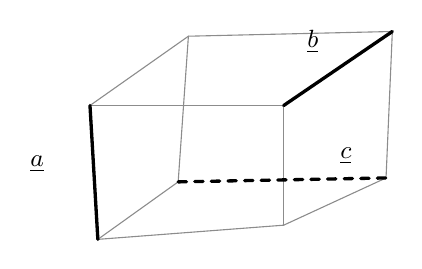
\begin{tikzpicture}[x=1mm,y=1mm,line cap=round,line join=round,font=\scriptsize]
\draw[pencil] (35,-29.6) -- (59.6,-29.6);
\draw[pencil] (59.6,-29.6) -- (59.6,-44.8);
\draw[pencil] (59.6,-44.8) -- (36,-46.6);
\draw[pencil] (47.5,-20.8) -- (73.4,-20.2);
\draw[pencil] (73.4,-20.2) -- (72.6,-38.8);
\draw[pencil] (46.2,-39.3) -- (47.5,-20.8);
\draw[pencil] (35,-29.6) -- (47.5,-20.8);
\draw[pencil] (59.6,-44.8) -- (72.6,-38.8);
\draw[pencil] (36,-46.6) -- (46.2,-39.3);
\draw[very thick] (35,-29.6) -- (36,-46.6);
\draw[very thick] (59.6,-29.6) -- (73.4,-20.2);
\draw[dashed,very thick] (46.2,-39.3) -- (72.6,-38.8);
\node[inner sep=1pt] at (28.3,-37) {\small $\underline{a}$};
\node[inner sep=1pt] at (63.3,-21.5) {\small $\underline{b}$};
\node[inner sep=1pt] at (67.5,-36) {\small $\underline{c}$};
\end{tikzpicture}
\end{document}
